

% !TEX root = ../popl-paper.tex
Reasoning about distributed message-passing applications is  hard. The degree of asynchrony
of the communication model is  an important ingredient of the application.
One reason
is that the communication architecture on which the application runs may vary, and must be accurately specified. In particular, an under-approximated communication model may hide safety errors,
such as unspecified receipts, whereas an over-approximated model may hide deadlocks. 

In synchronous communication (also known as rendez-vous communication), send and receive events are viewed as
a single event, i.e., a receive event and the corresponding send event happen simultaneously. The idea behind asynchronous communication, instead, is to decouple send and receive events, so that a receive event can happen indefinitely after the corresponding send event. By introducing some additional constraints on the execution of those events, we can obtain new communication models that sit somewhere between synchronous and fully asynchronous communication.
In this paper we try to clarify and classify some of these communication models.
%We consider only point-to-point communication, that is, messages that have exactly one sender and one receiver.
On  one hand, we consider communication models that were proposed in the early days of large-scale distributed computing to establish the correctness of some distributed algorithms, such as \emph{causal ordering}~\cite{Lamport78} for the correctness of Lamport's distributed mutual exclusion algorithm (see also~\cite{Renesse93}), or the weaker "FIFO" peer-to-peer assumption. On the other hand, we look at communication models that emerge
naturally when considering local-scale message-passing applications, which are based on predictable
message buffering supported by local FIFO queues (for instance "mailboxes"). Such communication models have
been considered in more recent works (for instance in~\cite{DBLP:journals/tcs/BasuB16}) and have caused
some confusion, specifically regarding the difference between causal ordering and mailboxes~\cite{DBLP:conf/cav/BouajjaniEJQ18,DBLP:conf/fossacs/GiustoLL20}.

The classification and axiomatisation of large-scale communication models received great attention in the late 90s~\cite{DBLP:journals/dc/Charron-BostMT96}, while the local-scale communication models have only started to be investigated quite recently by Chavrou~\emph{et al.}~\cite{DBLP:journals/fac/ChevrouHQ16}, focusing on a \emph{sequential} view of the behaviours of message-passing
applications (to be detailed below).
At the same time, several works~\cite{KraglQH18,GleissenthallKB19,DBLP:conf/cav/BouajjaniEJQ18,DBLP:conf/cav/LangeY19} recently addressed the verification of
asynchronous message-passing applications by reduction to their synchronous semantics (see also~\cite{Lipton75} for a seminal work on these questions). These results strongly rely on the ability to safely approximate an asynchronous communication model with a synchronous one. There is therefore a need to clarify how the synchronous-asynchronous spectrum of communication models is organised.

In this work, we start from the sequential hierarchy established by Chevrou~\emph{et al.}~\cite{DBLP:journals/fac/ChevrouHQ16}, where a
communication model is represented by a class of sequential executions; we revisit this hierarchy
with a non-sequential point of view: we define a communication model as a class of
\emph{Message Sequence Charts} (MSCs in the following).
Our MSCs are a graphical representation of computations of distributed systems, and they are a simplified
version of the ITU recommendation~\cite{messagesequencecharts}.
Roughly speaking, a distributed system is composed by a set of
sequential processes that can exchange messages. Each process executes a sequence of \emph{events}, which in our case will be either \emph{send}
or \emph{receive} events. A send event $s$ and a receive event $r$ are said to be \emph{matching} if the message sent by $s$ is the same  that is
received by $r$. 
A distributed computation is the \\
\noindent
concurrent execution of each process. In an MSC, such as the one in Fig.~\ref{fig:msc_ex}, each
vertical line is called a \emph{process line} and it represents the order in which events are executed by a single process, with time running from
top to bottom; arrows are used to represent messages and they connect a send event with the corresponding matching receive.
Given a message $m_i$, we will use $!i$ and $?i$ to denote the corresponding matching send and receive events, respectively. A single process line defines a
total order over the events executed by that process, i.e., an event $e$ happens before another event $e'$ if $e$ is higher in the process line;
in Fig.~\ref{fig:msc_ex}, if we look at process $q$ we see that $?1$ happens before $?2$. However, in general MSCs only specify a partial order
over events. Consider the events $!1$ and $!2$ in Fig.~\ref{fig:msc_ex}, which are executed by two different processes; these two events are \emph{truly concurrent}, in the sense that this MSC does not tell us which one is executed first.

\begin{wrapfigure}{r}{0pt}
	\begin{tikzpicture}[scale=0.8, every node/.style={transform shape}]
		\newproc{0}{p}{-2.5};
		\newproc{1}{q}{-2.5};
		\newproc{2}{r}{-2.5};

		\newmsgm{0}{1}{-0.5}{-0.5}{1}{0.5}{black};
		\newmsgm{2}{1}{-1.2}{-1.2}{2}{0.5}{black};
		\newmsgm{1}{0}{-1.9}{-1.9}{3}{0.5}{black};

		\newflechehorinverse{Purple}{-1.2}{2}{1};
		\newflechevert{Purple}{1}{-1.3}{-2.0};
		\newflechehorinverse{Purple}{-1.9}{1}{0};

		\newevent{black}{0}{-0.5}{!1}{left};
		\newevent{black}{1}{-0.5}{?1}{right};
		\newevent{black}{2}{-1.2}{!2}{right};
		\newevent{black}{1}{-1.2}{?2}{left};
		\newevent{black}{1}{-1.9}{!3}{below right};
		\newevent{black}{0}{-1.9}{?3}{left};

	\end{tikzpicture}
	\captionof{figure}{Red arrows between $!2$ and $?3$ denote a causal path.}
	\label{fig:msc_ex}
\end{wrapfigure}

\noindent Even though events on different processes can be concurrent, this is not always the case. For instance, a send event must always happen
before the matching receive event. Graphically, this \emph{happens before} relation between events on different processes is represented
by a path that follows the direction of the arrows and runs from top to bottom. This will be referred to as a \emph{causal path}, because it
estabilishes a causal relation between events. Fig.~\ref{fig:msc_ex} shows an example of causal path between the events $!2$ and $?3$. 
% Consider events $!1$ and $?2$ of the MSC shown in Fig.~\ref{fig:msc_ex}. Even though they are executed by different processes, $?2$ must happen
% before $!1$ because $?2$ must be executed after $!2$, which happens before $?1$, which in turn happens before $!1$.
% The fact that $!1$ is higher on his own process line compared to $!2$ does not meaning anything with respect to the order in which they are
% executed.


% Since an MSC defines a partial order over the events of a distributed system, it can always be extended to a total order, which will be referred to as a \emph{linearization}.
% %Given an MSC, it can have multiple linearizations. For the MSC in Fig.~\g:msc_ex}, both $!1\;?1\;!2\;?2$ and $!2\;!1\;?1\;?2$ are valid linearizations, i.e. a total order over the events which is compatible with the partial order defined by the MSC.
% Intuitively, a linearization represents the order in which events are executed by the distributed system according to \emph{absolute time}, i.e. as they are seen by an external viewer that has a global view of all the processes.




As mentioned before, in this work we interpret communication models as classes of MSCs.
This non-sequential view of the communication models is arguably the "standard one",
rather than the sequential point of view adopted by Chevrou~\emph{et al}. It is more relevant for comparing communication models, as some
of them, such as causally ordered communications, intrinsically rely on this non-sequential view and the happens-before relation. Large-scale communication models are quite easy to axiomatize in a formal language, such as monadic second order logic (MSO) over MSCs. Local-scale
communication models, on the other hand, are easy to define by means of an operational semantics involving FIFO queues, but their axiomatization
in MSO is error prone and requires particular attention. The choice of MSO as a specification language for the axiomatisation of
these communication models is not incidental: there is a wealth of results on MSO model-checking over MSCs that originated from
the work of Genest~\emph{et al.}~\cite{genest2004kleene,GKM07}, with recent developments by Bollig~\emph{et al.} in the context
of synchronisability~\cite{BolligGFLLS21}.

\etienne{Do we really want to repeat Fig2 at Fig8? By the way Fig2 is not the up to date version of Fig8}

Our contributions are the following:
\begin{itemize}
	\item We review the peer-to-peer FIFO, causally ordered, mailbox, \onen, \nn, asynchronous, and synchronous communication models
	and propose definitions of these models in terms of classes of MSCs. For the communication models whose intuition stems from
	an operational semantics, we provide an alternative operational definition, and we show soundness and completeness.

	\item From these definitions, we deduce a new non-sequential hierarchy of communication models (see Fig.~\ref{fig:msc_hierarchy_full})
	and establish the strictness of this hierarchy by means of several examples.
	Surprisingly, the \onen class, that could be thought of as the "dual" of the mailbox class, is a subclass of mailbox class. This strongly
	contrasts with Chevrou~\emph{et al.} sequential hierarchy, where \onen and mailbox are incomparable. The comparison between
	the \onen and mailbox classes is non-trivial in our non-sequential setting, and it motivates the introduction
	of several technical alternative characterisations of these communication models.

	\item We show that all of these communication models can be axiomatised in MSO. This result is rather subtle for mailbox and \onen, and highly non-trivial for \nn. For the latter, we develop a constructive proof based on an
	algorithm that computes a \nn linearisation of an MSC.

	\item Building on the MSO characterization of these communication models, we derive several new decidability results (cfr. Fig. \ref{fig:stw-boundshort}) for bounded
	model-checking of systems of communicating finite state machines under various bounded assumptions (existential boundedness, weak synchronisability, etc).
\end{itemize}



\begin{figure}[t]
	\captionsetup[subfigure]{justification=centering}
	% \centering
%	
	\begin{subfigure}{0.3\textwidth}\centering	
	\begin{tikzpicture}[scale=0.78, every node/.style={transform shape}]
		\draw  (0,0) rectangle (1.5,.6);
		\draw (1.5,0.3) node[left]{\rsc};
		\draw  (0,0) rectangle (2.1,1.2);
		\draw (2.1,0.9) node[left]{\nn};
		\draw  (0,0) rectangle (2.7,1.8);
		\draw (2.7,1.5) node[left]{\onen};
		\draw  (0,0) rectangle (3.3,2.4);
		\draw (3.3,2.1) node[left]{\mb};
		\draw  (0,0) rectangle (3.9,3);
		\draw (3.9,2.7) node[left]{\co};
		\draw  (0,0) rectangle (4.5,3.6);
		\draw (4.5,3.3) node[left]{\pp};
		\draw  (0,0) rectangle (5.1,4.2);
		\draw (5.1,3.9) node[left]{\asy};
	\end{tikzpicture}
	\caption{The hierarchy of MSC classes.\\ ~}
	\label{fig:msc_hierarchy_full}
	\end{subfigure} \quad   
	\begin{subfigure}{0.65\textwidth}\centering
	{\small
		\begin{tabular}{| c | c | c|  c| c| } 
			\hline
			& Weakly  & Weakly  & $\exists$k & $\forall$k  \\
			& sync & k-sync & bounded & bounded \\
			\hline \hline
			$\asy$ &  \xmark & \cmark & \cmark & \cmark \\
			\hline
			$\oneone$  & \xmark~[1] & \cmark~[1] & \cmark~[1] & \cmark~[1] \\
			\hline
			$\co$  & \xmark & \cmark & \cmark & \cmark \\
			\hline
			$\none$ & \cmark~[1] & \cmark~[1] & \cmark~[1] & \cmark~[1] \\
			\hline
			$\onen$ & \cmark & \cmark & \cmark & \cmark \\
			\hline
			$\nn$ & \cmark & \cmark & \cmark & \cmark \\
			\hline
		%	$\rsc$ & \cmark & \cmark & \cmark & \cmark & \cmark \\
		%	\hline
		\end{tabular}
		}
		\caption{ (Un)decidability results for the synchronisability problems, %(each 
		%combination of a communication model $\comsymb$ and a class $\aMSCclass$ of MSCs is a different 
		%synchronisability problem). 
		%The symbol \xmark\;stands for undecidability and unbounded special tree-width
	%	of $\comsymb\cap \aMSCclass$, whereas \cmark\;stands for decidability and bounded STW
%		of $\comsymb\cap \aMSCclass$.  
		[1] indicates that the result was shown in \cite{BolligGFLLS21}.}
		\label{fig:stw-boundshort}
\end{subfigure}
\caption{Main contributions}
	%\etienne{Maybe move that figure later? end of section 2? section 6?}
\end{figure}

\paragraph{\bf Outline} The paper is organized as follows. Section~\ref{sec:MSC} describes the communication models we consider. We also recall the notion of MSC and introduce formal definitions for these models, seen as classes of MSCs.
In Section~\ref{sec:impl}, we rely on
an operational semantics to provide an alternative definition for some of these communication models, which we prove to be sound and complete.
Section~\ref{sec:MSO} characterizes the classes of MSCs via MSO logic.
In Section~\ref{sec:hierarchy}, we compare all of the considered communication models and show our main result: a strict non-sequential hierarchy of communication models.
Finally, Section~\ref{sec:checking} shows some (un)decidability results for various bounded model-checking
problems based on MSO and on the notion of special treewidth.


%\hrule
%
%\bigskip
%
%\etienne{Below: keep in the intro, move elsewhere, or drop}
%
%Consider the events $!1$ and $!2$ in Fig.~\ref{fig:msc_ex}, which are executed by two different processes; these two events are said to be \emph{concurrent}, in the sense that this MSC does not tell us which one is executed first.
%
%generalize the models to  consider unmatched messages (i.e., messages that have been sent, but not yet read).
%MSCs are a graphical representation of the  computations of distributed systems.  Roughly speaking, a distributed system is composed by a set of sequential processes that can exchange messages. Each process exhibits a sequence of \emph{events}, which in our case will be either \emph{send} or \emph{receive} events. A send event $s$ and a receive event $r$ are said to be \emph{matching} if the message sent by $s$ is the same  that is received by $r$. A distributed computation is the concurrent execution of each process. In an MSC, such as the one in Fig.~\ref{fig:msc_ex}, each vertical line is called a \emph{process line} and it represents the order in which events are executed by a single process, with time running from top to bottom; arrows are used to represent messages and they connect a send event with its corresponding matching receive.
%Given a message $m_i$, we will use $!i$ and $?i$ to denote the corresponding two matching send and receive events. A single process line defines a total order over the events executed by that process, i.e., an event $e$ happens before another event $e'$ if $e$ is higher in the process line; in Fig.~\ref{fig:msc_ex}, if we look at process $q$ we see that $?1$ happens before $?2$. However, in general MSCs only specify a partial order over events.
%
%
%\cinzia{Have a look at \url{https://web.archive.org/web/20060826195305/http://www.comp.nus.edu.sg/~thiagu/public_papers/surveymsc.pdf}}
%
%\cinzia{\url{https://link.springer.com/content/pdf/10.1007/978-0-387-35271-8.pdf} to mention while talking about realizability page 81-96}
%
%Going back to our contribution, the work in \cite{DBLP:journals/fac/ChevrouHQ16} describes the properties that a single linearization must satisfy in order to be realizable by a system that uses a given communication model. On the other hand, we are interested in understanding if a given MSC describes a computation that can be realized by a system that uses some communication model $CM$. In other words, given a MSC we want to know if it has at least one linearization that respects the constraints imposed by $CM$. If that is the case, the MSC represents a behaviorthat can be exhibited by a system that uses $CM$ as a communication model. These are two fundamentally dissimilar problems; at the end of this section we provide an example to clarify the difference. In our work, we are going to formally characterize the classes of MSCs which represent valid computations for all of these seven communication models. We also show how these classes form a well-defined hierarchy, which does not correspond entirely to that found in \cite{DBLP:journals/fac/ChevrouHQ16}.

%\cinzia{talk about realizations here?}
%
%\cinzia{say that the two hierarchy differs}
%\paragraph{Contributions.}\cinzia{to rewrite here}
%
%We find of particular interest to study the relation between the classes of MSCs for all of these communication models. For instance, the MSC shown in Fig.~\ref{fig:co_ex} is both asynchronous and $\oneone$, in the sense that we are able to find systems using those communication models that can produce the behaviordescribed by the MSC. Is it always the case than a $\oneone$ MSC is also an asynchronous MSC? What about the other communication models? In Section~\ref{sec:hierarchy} we prove that the classes of MSCs for all these communication models form a very neat hierarchy, which is graphically shown in Fig.~\ref{fig:msc_hierarchy_full}.

% \cinzia{redo fig in tikz}
% \begin{figure}[h]
% 	\centering
% 	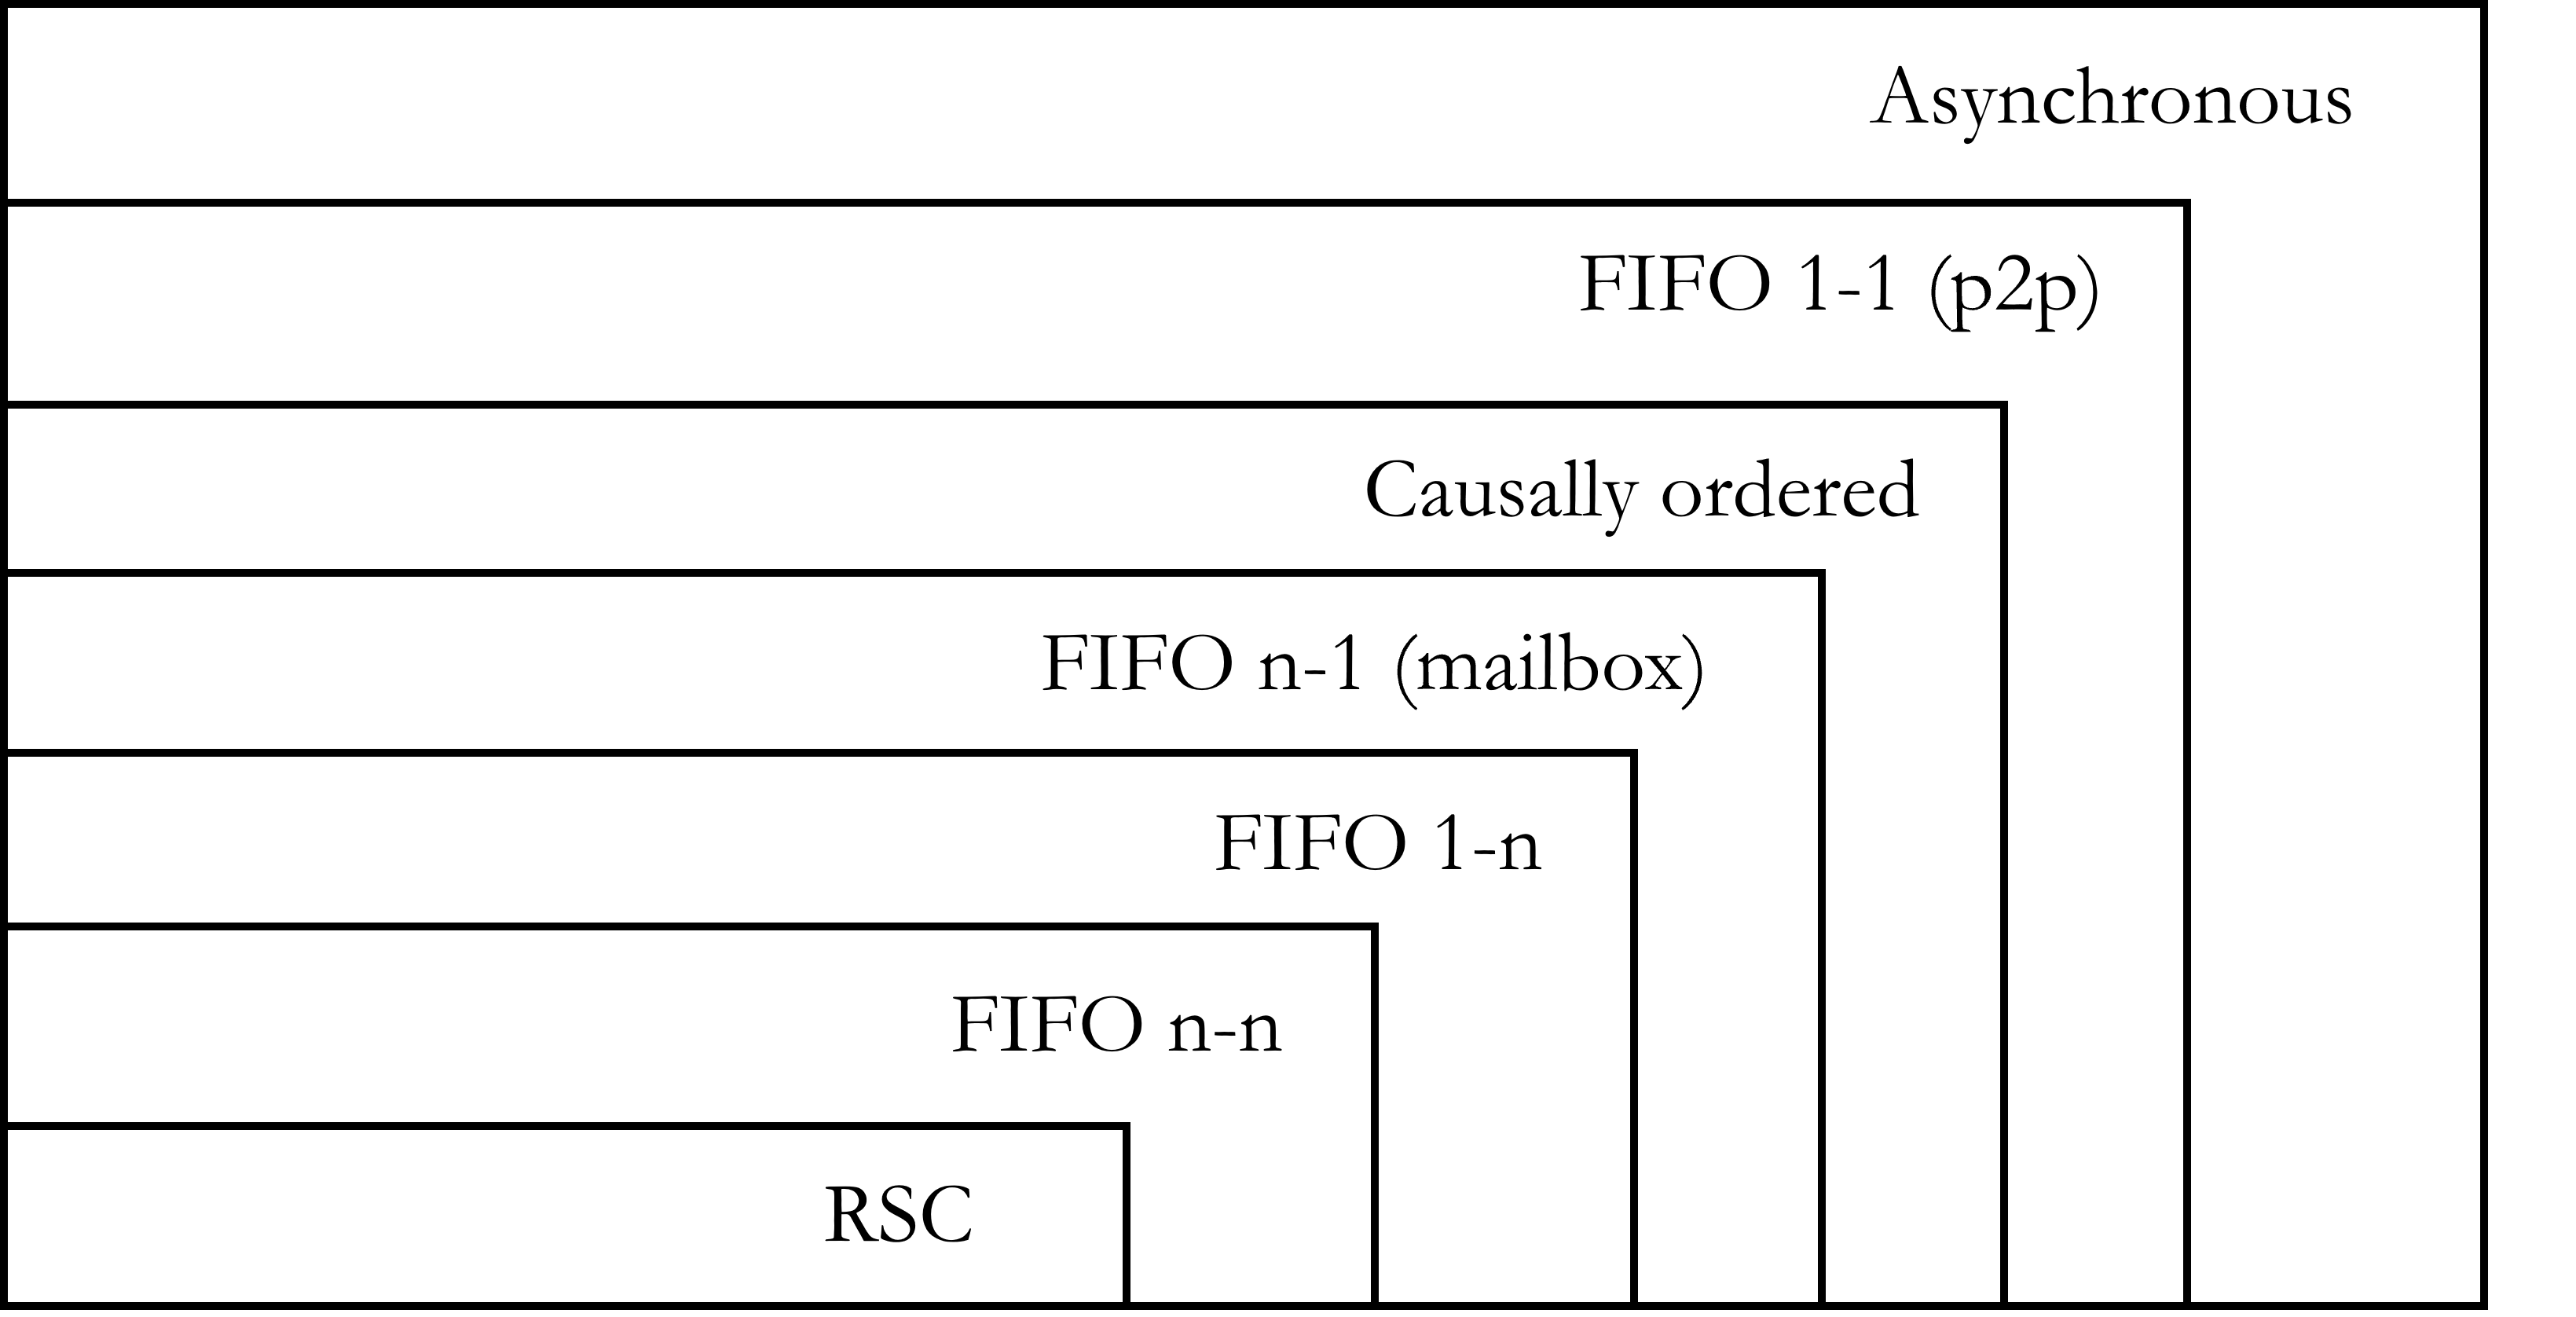
\includegraphics[width=8cm]{msc_hierarchy}
% 	\caption{The hierarchy of MSC classes.}
% 	\label{fig:msc_hierarchy_full}
% \end{figure}



